\subsection{Ablation Study}
\label{sec-eval-ablation}


In this subsection, we conduct an ablation study on different aspects on \sysname. In particular, we are interested in answering the following two questions: 1) what is the effect of chunking on prefill throughput, and 2) analyzing the impact of hybrid-batching and chunking on latency. While we provide results only for a few experiments in this section, all the trends discussed below are consistent across various model-hardware combinations.

\subsubsection{Overhead of \chunking}
\label{sec-eval-ablation1}

\autoref{fig:eval:ablation:overheads} shows how much overhead chunking adds in \yi{} -- on overall prefill runtime. As expected, smaller chunks introduce higher overhead as shown by the gradually decreasing bar heights in~\autoref{fig:eval:ablation:overheads}. However, even with the smallest chunk size of 512, we observe a moderate overhead of at most $\sim$25\%. Whereas with the larger token budget of 2048, chunked prefills have almost negligible overhead. %









\begin{figure}[t!]
    \centering        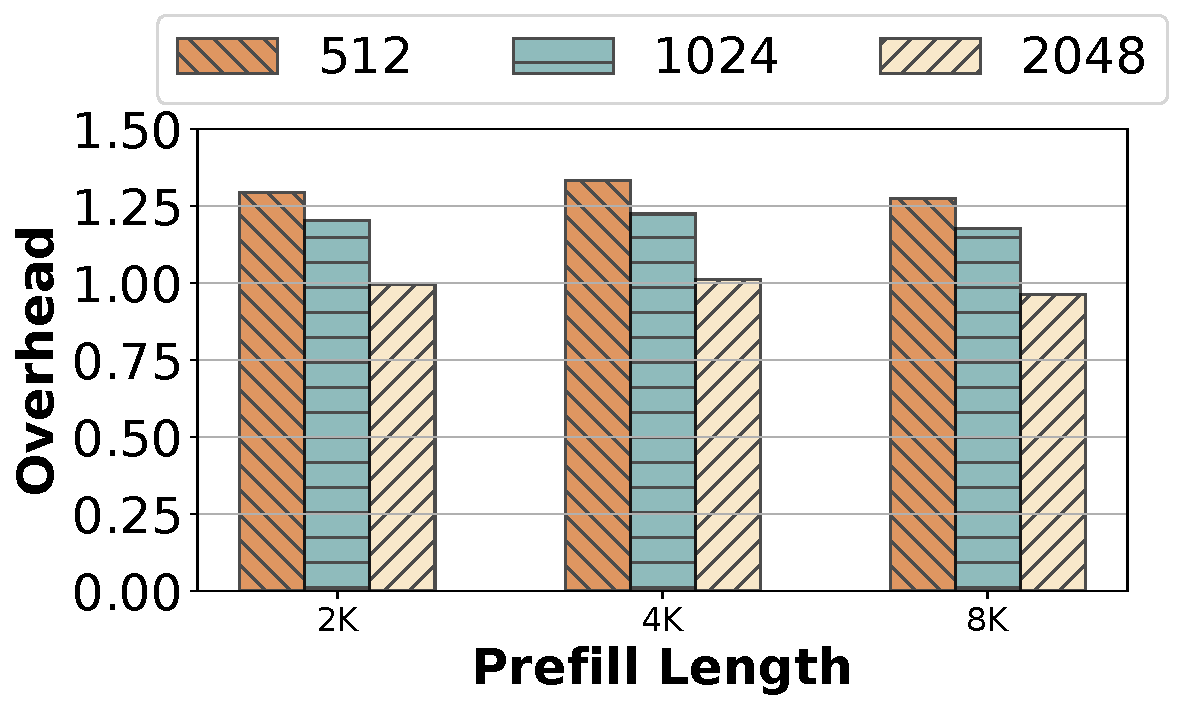
\includegraphics[width=0.38\textwidth]{figures/chunking-overhead.pdf}
    \caption{Overhead of \chunking in prefill computation for Yi-34B (TP-2) normalized to the cost of no-chunking, shown for various prompt lengths using chunk lengths of 512, 1024 and 2048.}
    \label{fig:eval:ablation:overheads}
\end{figure}



\begin{table}[t]
\centering
\setlength{\tabcolsep}{2pt}
\scalebox{0.85}{
\begin{tabular}{c|cc|cc}
\textbf{Scheduler} & \multicolumn{2}{c|}{\textbf{\sharegpt}} & \multicolumn{2}{c}{\textbf{\arxivsum}} \\
\cline{2-3} \cline{4-5}
& P50 TTFT & P99 TBT & P50 TTFT & P99 TBT \\ \toprule
\dcoel{}\textit{-only} & 0.53 & 0.68 & 3.78 & 1.38 \\
\chunking{}\textit{-only} & 1.04 & 0.17 & 5.38 & 0.20 \\
\sysname (combined) & 0.76 & 0.14 & 3.90 & 0.17 \\
\bottomrule
\end{tabular}}
\caption{TTFT and TBT latency measured in seconds for \dcoel and \chunking used in isolation as well as when they are used in tandem, evaluated over 128 requests for Yi-34B running on two A100s with a token budget of 1024. By using both \dcoel and \chunking, \sysname is able to lower both TTFT and TBT.}
\label{table:eval:attribution}
\end{table}


\subsubsection{Impact of individual techniques}
\label{sec-eval-ablation2}
Finally, \autoref{table:eval:attribution} shows the TTFT and TBT latency with each component of  \sysname evaluated in isolation \ie \chunking-only, \dcoel-only (mixed batches with both prefill and decode requests) and when they are used in tandem. These results show that the two techniques work best together: \chunking-only increases TTFT as prefill chunks are slightly inefficient whereas \dcoel-only increases TBT because long prefills can still create generation stalls. When used together, \sysname improves performance along both dimensions.
